\chapter{Анализ предметной области}

В данном разделе определяются основные определения, используемые при анализе, а также описывается актуальность исследуемой области.

\section{Использование логического программирования}
Математическая логика является формализацией человеческого мышления и представления знаний. В связи с целью автоматизации процесса логического вывода возникла новая парадигма --- логическое программирование. В основе этой идеи лежит описание задачи совокупностью утверждений на некотором формальном логическом языке и получение решения с помощью вывода в некоторой формальной системе \cite{logic_researchers1}.

В широком смысле логическое программирование представляет собой семейство таких методов и решений проблем, в которых используются приемы логического вывода для манипулирования знаниями. В узком -- использование исчисления предикатов первого порядка в качестве основы для описания предметной области с использованием дизъюнктов Хорна \cite{horn_disjunction}.  

Машина логического вывода --- реализованная программным или аппаратным образом высокоуровневая абстракция, выполняющая генерацию новых фактов и правил в соответствии с законами формальной логики \cite{machine_logic_output}. Используемые в ней архитектурные решения определяют задачу логического вывода. 

Известным языком программирования в данной парадигме является Prolog и его реализации \cite{prolog}. Программа состоит из набора фактов, а также отношений, которые устанавливаются между ними. Существует некоторая база данных, в которой они хранятся вместе с задаваемыми правилами. Для начала выполнения работы программа должна иметь запрос. Он образуется из термов, каждый из которых должен иметь истинное значение.

Использование логического программирования привлекает разработчиков тем, что программы не содержат затрудняющие для понимания детали, а описывают то, что собой представляет результат решения; данная особенность позволяет проще осуществить проверку и убедиться в том, что реализуется требуемое.


\section{Параллелизм}
Ввиду того, что определенные этапы вычислений могут производиться параллельно, то должна быть заложена возможность распределения подзадач между несколькими исполнителями.

Логическое программирование предлагает некоторые возможности для неявного использования параллелизма. Выделяют два основных вида параллелизма: AND-параллелизм и OR-параллелизм \cite{parallel_logic}.

\textit{Независимый OR-параллелизм} основан на параллельном выполнении дизъюнкции предикатов, не имеющих общих переменных. Результат будет получен из первого выполнившегося терма. Это соответствует параллельному просмотру дерева поиска (OR-дерева). Пример OR-параллелизма представлен на рисунке \ref{image:or_parallelism}.

\begin{figure}[H]
	\centering{
		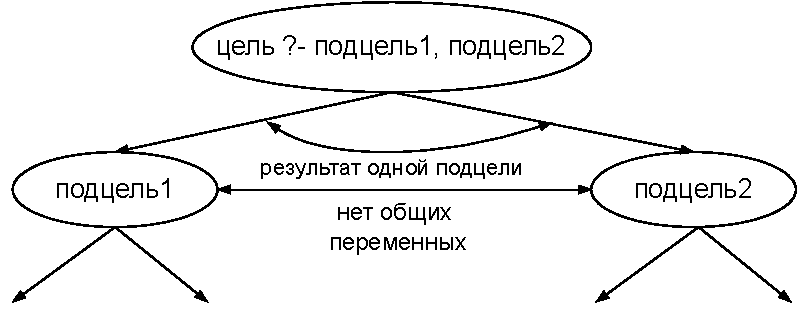
\includegraphics[scale=1]{images/or_parallelism.pdf}
		\caption{Пример OR-параллелизма.}
		\label{image:or_parallelism}}
\end{figure} 

\newpage

В основе идеи \textit{независимого AND-параллелизма} лежит распараллеливание конъюнкции подцелей, которые не имеют одни и те же переменные. Такие термы не будут влиять на выполнение друг друга, устраняя необходимость введения какой-либо формы синхронизации во время параллельного выполнения. Данный способ проиллюстрирован на рисунке \ref{image:and_parallelism}. 

\begin{figure}[H]
	\centering{
		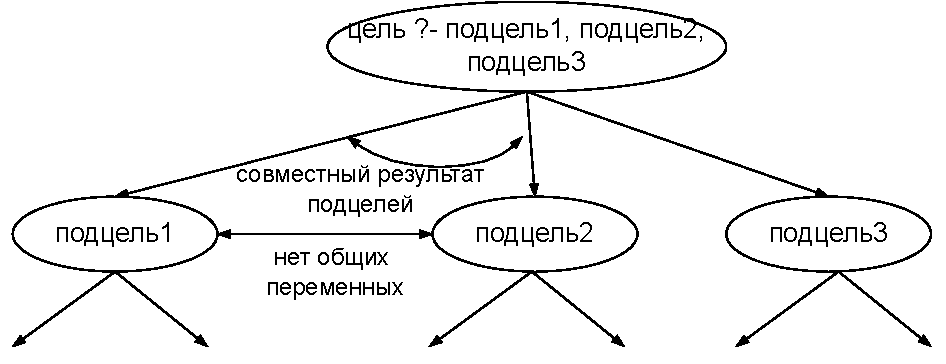
\includegraphics[scale=1]{images/and_parallelism.pdf}
		\caption{Пример AND-параллелизма.}
		\label{image:and_parallelism}}
\end{figure} 

\textit{Зависимый AND-параллелизм} возникает, когда задается конъюнктивная цель вида $p (X)\ \&\ q (X)$ --- две подцели выполняются параллельно, но при этом используют общую переменную.

Развитие идей Prolog привело к созданию таких языков, как Datalog \cite{datalog}, Yedalog \cite{yedalog} и др. 
\textit{Datalog} --- декларативный язык программирования, который синтаксически является подмножеством Пролога. Программа Datalog состоит из конечного числа фактов и правил. Они задаются с помощью атомарных формул, которые состоят из предикатов с аргументами (листинг \ref{datalog}). В \textit{зависимом OR-параллелизме} выполняется дизъюнкция цели с общей переменной. 
\newpage
\begin{lstlisting}[label = datalog, caption=Пример описания отношений с использованием Datalog, numbers = none]
	father relational table
	- - - - - - - - - - - -
	harry    john
	john     david

	FACTS
	father(harry, john).
	father(john, david).
	
	RULE
	grandfather(Z, X) :- father(Y, X), father(Z, Y).
\end{lstlisting}

Полученные в последние двадцать пять лет результаты в теории параллельного логического вывода (В. Ю. Мельцов, А. И. Симонов \cite{logic_researchers_3}; М. Н. Томчук, Д. А. Страбыкин, Е. В. Агалаков \cite{logic_researchers_4} и др.) позволяют вплотную подойти к реализации методов и машин логического вывода на высокопроизводительных многопроцессорных системах как с общей, так и с распределенной памятью. 

\section{Вывод}
Описано введение в предметную область логического вывода. Приведены определения, которые в дальнейшем будут использованы при обзоре способов использования параллелизма. 